%tirar o anonymous dps
\documentclass[sigconf]{acmart}
\renewcommand{\figurename}{Figura}
\renewcommand{\tablename}{Tabela}

\acmConference[ISE 2026]{5th Brazilian Workshop on Intelligent Software Engineering}{September 11, 2026}{São Paulo, SP, Brazil}
\usepackage{tikz}
\usetikzlibrary{shapes.geometric, arrows.meta, positioning, calc}
%% Using the option "anonymous" will produce "Anonymous Author(s)"
%% for double-anonymized review. Upon acceptance, remove this option
%% and set the authors' names and affiliations using the corresponding
%% commands.

%% CBSoft uses an ACM-like format without the ACM Reference block.
%% The following warning from acmart can be safely ignored:
%% "ACM reference format is mandatory for papers over one page."
\settopmatter{printacmref=false}
\renewcommand\footnotetextcopyrightpermission[1]{} % 

\setcopyright{none}


\AtBeginDocument{
    \providecommand\BibTeX{{Bib\TeX}}
}

\begin{document}





%%pensar em um titulo melhor depois 
\title{Um pipeline híbrido para detecção inteligente e confiável de bugs e code smells em Python}

%% The "author" command and its associated commands are used to define
%% the authors and their affiliations.
%% Of note is the shared affiliation of the first two authors, and the
%% "authornote" and "authornotemark" commands



%%
% \author{Fernanda Alice Duarte}
% \affiliation{
%   \institution{ Instituto de Computação (Icomp) - Universidade Federal do Amazonas (UFAM)}
%   \city{Manaus}
%   \country{Brasil}
% }
% \email{fernanda.duarte@icomp.ufam.edu.br}
%
% \author{Rosiane de Freitas}
% \affiliation{
%   \institution{ Instituto de Computação (Icomp) - Universidade Federal do Amazonas (UFAM)}  \city{Manaus}
%   \country{Brasil}
% }
% \email{rosiane@icomp.ufam.edu.br}
%
% \author{Lucas C. Cordeiro}
% \affiliation{
%   \institution{University of Manchester}
%   \city{Manchester}
%   \country{UK}
% }
% \email{lucas.cordeiro@manchester.ac.uk}
%
% %% By default, the full list of authors will be used on the page
% %% headers. This list is often too long and will overlap
% %% other information printed in the page headers. 
% %% This command allows the author to define a more concise list
% %% of authors' names for this purpose.
% \renewcommand{\shortauthors}{Duarte et al.}

\renewcommand{\shorttitle}{Pipeline Híbrido LLM+ESBMC-Python}

%% Artigo escrito em português: usar os cabeçalhos em português.
\renewcommand\abstractname{Resumo}
\renewcommand\keywordsname{Palavras-chave}
\renewcommand\refname{Referências}

%%revisar o resumo
\begin{abstract}
Python é uma das linguagens mais utilizadas atualmente, mas sua natureza dinâmica dificulta a aplicação de verificação formal. O ESBMC-Python, um verificador formal baseado em \textit{bounded model checking}, verifica programas Python, enquanto modelos de linguagem (LLMs e SLMs) apoiam a revisão de código, ainda que sujeitos a falsos positivos e alucinações. Este trabalho propõe um pipeline híbrido em que um modelo de linguagem realiza a triagem inicial de funções em Python; uma etapa de validação estrutural via AST descarta achados que não correspondem a expressões reais do código, e o ESBMC-Python confirma formalmente apenas os bugs verificáveis, restrito a três categorias de bugs e três categorias de \textit{code smells}. Uma avaliação preliminar em um dataset de 70 funções em Python, comparando cinco modelos (três via API e dois locais via Ollama), mostra que o pipeline híbrido aumenta a precisão de todos os modelos avaliados em relação ao uso isolado da LLM, com Taxa de Redução de Ruído entre 0.500 e 1.000, sendo o ganho mais expressivo nos modelos locais. A validação por AST também filtra alucinações estruturais observadas exclusivamente nos modelos locais. Os resultados indicam que a abordagem é orientada ao aumento de precisão e não de revocação.
\end{abstract}

%% Keywords. The author(s) should pick words that accurately describe
%% the presented work. Separate the keywords with commas.
\keywords{verificação formal, modelos de linguagem, IA generativa, ESBMC, detecção de falhas, Python, code smells}

%% This command processes the author, affiliation, and title
%% information and builds the first part of the formatted document.
%% "frenchspacing" avoids an additional space after a period at the end of a sentence.
\frenchspacing
\maketitle

\section{Introdução}

Python é amplamente empregado no desenvolvimento de aplicações em diferentes domínios \cite{tiobe2026}. Com a crescente adoção da linguagem, torna-se cada vez mais importante avaliar a qualidade do código produzido, não apenas em termos de estilo e manutenibilidade, mas também quanto à presença de bugs capazes de comprometer seu comportamento.

Entretanto, a natureza dinâmica do Python dificulta análises mais precisas e a aplicação de técnicas de verificação formal. Nesse contexto, o ESBMC-Python introduziu suporte à verificação de programas Python por meio de bounded model checking, permitindo a análise formal de propriedades como violações de asserções, erros aritméticos e acessos inválidos~\cite{farias2024esbmcpython}.

Paralelamente, modelos de linguagem têm sido cada vez mais utilizados para apoiar atividades de revisão e análise de código. Embora apresentem resultados promissores na identificação de possíveis defeitos, esses modelos ainda podem produzir falsos positivos, respostas inconsistentes e justificativas incorretas, especialmente em cenários mais próximos de aplicações reais~\cite{ullah2024secllmholmes,ding2025primevul}.

Por outro lado, a aplicação da verificação formal em larga escala em projetos maiores pode apresentar limitações de escalabilidade devido ao custo computacional, ao tempo de processamento e à necessidade de selecionar e preparar os trechos de código que serão analisados~\cite{shivaji2026eva}.

Diante desse cenário, a contribuição deste trabalho é um pipeline híbrido no qual um modelo de linguagem realiza a triagem inicial de funções Python, classificando potenciais bugs e code smells; uma etapa de validação estrutural verifica a consistência das hipóteses geradas; e o ESBMC-Python confirma formalmente apenas os bugs verificáveis.

\section{Trabalhos Relacionados}
 O ESBMC-Python permite verificar diretamente programas em Python anotados com tipos, eliminando a necessidade de tradução para outra linguagem~\cite{farias2024esbmcpython}. Em contraste, o PyVeritas utiliza uma LLM para transpilar o código Python para C e, posteriormente, realiza a verificação com o CBMC~\cite{orvalho2025pyveritas}. De forma semelhante, o EVA emprega uma LLM para traduzir programas Python para C antes da análise pelo ESBMC tradicional~\cite{shivaji2026eva}. Diferentemente dessas abordagens, este trabalho visa utilizar a LLM apenas para a triagem inicial de possíveis defeitos, preservando o código Python original para a verificação direta pelo ESBMC-Python.

Embora modelos de linguagem apresentem resultados promissores na análise
de código, eles ainda podem produzir falsos positivos, respostas
inconsistentes e justificativas incorretas~\cite{ullah2024secllmholmes,ding2025primevul}. Por outro lado, a verificação formal baseada em Bounded Model Checking pode confirmar ou refutar propriedades do programa dentro dos limites de verificação considerados, produzindo contraexemplos quando uma violação é encontrada, embora apresente desafios relacionados ao custo computacional e à escalabilidade. Nesse contexto, Tihanyi et al.~\cite{tihanyi2025vulnerability} defendem abordagens híbridas que exploram a alta cobertura proporcionada pelas LLMs juntamente com a confiabilidade oferecida pela verificação formal.

Além da detecção de bugs executáveis, modelos de linguagem também vêm sendo empregados na identificação de \textit{code smells}. Santos et al.~\cite{santos2023yetanothermodel} identificaram atributos estruturais compartilhados por modelos de predição de defeitos e de diferentes \textit{code smells}, especialmente relacionados à complexidade, à documentação e ao tamanho. Complementarmente, Souza et al.~\cite{souza2026beyondstrictrules} observam que o desempenho das LLMs varia conforme o tipo de \textit{code smell} analisado. Paralelamente, modelos menores (\textit{Small Language Models}, SLMs) vêm sendo avaliados em tarefas de engenharia de software: Gheyi et al.~\cite{gheyi2025slms} avaliam especificamente a eficácia de SLMs na detecção de bugs de refatoração e observam desempenho fortemente dependente do modelo e da tarefa, uma instabilidade também observada nos modelos locais deste trabalho (Seção~\ref{sec:resultados}). Essa distinção orienta o tratamento diferenciado do pipeline: bugs são hipóteses candidatas à confirmação formal, e \textit{code smells} ficam sujeitos ao julgamento do modelo, sem verificação executável equivalente.

\section{Pipeline Híbrido}

O pipeline proposto analisa funções Python em cinco etapas.
Inicialmente, o código-fonte é convertido em uma Árvore Sintática
Abstrata (\textit{Abstract Syntax Tree} -- AST), uma representação
estruturada da sintaxe do programa. Essa representação preserva os
elementos sintáticos da função e é utilizada posteriormente para validar
estruturalmente as hipóteses geradas pelo modelo de linguagem.

Nesta avaliação inicial, o escopo foi limitado a seis categorias: três
bugs verificáveis formalmente (\textit{division by zero},
\textit{out-of-bounds access} e \textit{assertion violation}) e três
\textit{code smells} amplamente reconhecidos na literatura de
refatoração~\cite{fowler1999refactoring} (\textit{long method},
\textit{many parameters} e \textit{complex conditional}).

\begin{figure}[htb]
  \centering
  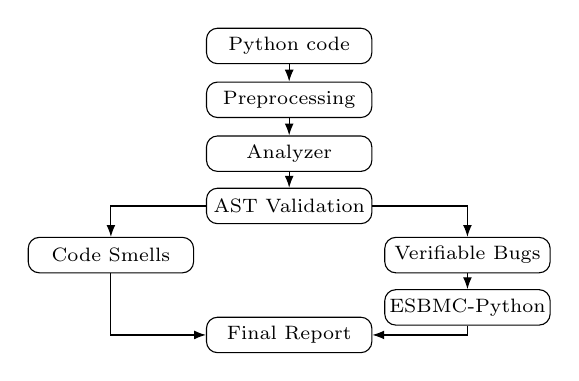
\begin{tikzpicture}[
      node distance=1.3mm and 2mm,
      box/.style={rectangle, draw, rounded corners, align=center,
                  minimum width=2.1cm, minimum height=4.5mm,
                  font=\scriptsize, inner sep=1.5pt},
      arr/.style={-{Latex[length=1.5mm]}}
    ]

    \node[box] (input) {Python code};
    \node[box, below=2.2mm of input] (pre) {Preprocessing};
    \node[box, below=2.2mm of pre] (llm) {Analyzer};
    \node[box, below=2mm of llm] (ast) {AST Validation};

    \node[box, below left=1.6mm and 1.5mm of ast] (smell) {Code Smells};
    \node[box, below right=1.6mm and 1.5mm of ast] (bug) {Verifiable Bugs};
    \node[box, below=2mm of bug] (esbmc) {ESBMC-Python};

    \node[box, below=4.5mm of $(smell)!0.5!(esbmc)$] (report) {Final Report};

    \draw[arr] (input) -- (pre);
    \draw[arr] (pre) -- (llm);
    \draw[arr] (llm) -- (ast);
    \draw[arr] (ast) -| (smell);
    \draw[arr] (ast) -| (bug);
    \draw[arr] (bug) -- (esbmc);
    \draw[arr] (smell) |- (report);
    \draw[arr] (esbmc) |- (report);

  \end{tikzpicture}
  \caption{Visão geral do pipeline híbrido proposto.}
  \label{fig:pipeline}
\end{figure}


O pipeline converte o arquivo \texttt{.py} em uma AST por meio do módulo
\texttt{ast} da linguagem Python. Cada função é transformada em um objeto da classe \emph{CodeUnit}, que
organiza parâmetros, anotações de tipo, operações, laços e condicionais. A AST original é preservada para uso na etapa de
AST Validation.

Cada \emph{CodeUnit} é enviado ao modelo por meio de um prompt estruturado
com \emph{persona prompting} (especialista em segurança de código Python),
que auxilia na mitigação de alucinações~\cite{ullah2024secllmholmes}, e
\emph{Chain-of-Thought} (CoT), que decompõe a análise em etapas lógicas e
melhora a organização do
veredito~\cite{ullah2024secllmholmes,souza2026beyondstrictrules,tihanyi2025vulnerability},
orientando uma análise passo a passo das
operações potencialmente perigosas antes da classificação. O prompt orienta
o modelo a sinalizar candidatos mesmo diante de guardas que pareçam
parciais, deixando essa determinação para a etapa de verificação formal;
funções sem problemas identificados retornam uma lista de achados vazia. A
saída segue um schema JSON restrito às seis categorias consideradas neste
estudo, com a flag \texttt{verifiable} e uma curta justificativa. Em
seguida, a AST Validation verifica se os achados reportados correspondem a
expressões existentes no código; caso a expressão não seja encontrada na
AST, o achado é descartado como uma alucinação estrutural~\cite{khati2026forge}.

Achados com a flag \texttt{verifiable=true} são encaminhados ao
ESBMC-Python, enquanto \textit{code smells} e demais achados não
verificáveis seguem diretamente para o relatório final. A função original é
analisada pelo ESBMC-Python, restrita à função-alvo, com verificação
incremental e atribuição não determinística aos parâmetros de entrada; o
verificador confirma a hipótese quando encontra uma violação dentro do
limite configurado, gerando um contraexemplo, e não a confirma na ausência
de contraexemplo. O relatório final consolida, para cada função, o
resultado produzido pelo modelo, o veredito do ESBMC-Python e o rótulo de
\textit{ground truth} do dataset, exportando os dados em formato JSON para
o cálculo das métricas apresentadas na próxima seção.






\section{Avaliação Preliminar}
\subsection{Configuração Experimental}

O dataset utilizado é composto por 70 funções Python: 45 contêm bugs
executáveis (15 por categoria, totalizando 48 instâncias de defeito,
já que \textit{out-of-bounds} pode ocorrer mais de uma vez por
função), 15 contêm \textit{code smells} (5 por categoria) e 10 são
funções limpas, usadas como controle negativo. O rótulo correto de
cada função (\textit{ground truth}) foi anotado manualmente em arquivos
JSON e validado por meio da execução direta do ESBMC-Python sobre cada
arquivo (Flow A), confirmando que todas as 48 instâncias de defeito
eram alcançáveis e foram identificadas pelo verificador
(P=R=F1=1.000).

Foram comparados três fluxos de execução:
\textbf{Flow A}, execução direta do ESBMC-Python, utilizada apenas para
validar o dataset; \textbf{Flow B}, pipeline híbrido proposto, composto
pela triagem do modelo de linguagem, validação estrutural por AST e
confirmação formal pelo ESBMC-Python; e \textbf{Flow C}, uso isolado do
modelo de linguagem, sem confirmação formal. O Flow A não é tratado
como abordagem concorrente, sendo empregado apenas como teste de
sanidade para verificar a alcançabilidade dos defeitos anotados. Embora
o mesmo verificador seja utilizado no Flow A e no Flow B, essa
circularidade é mitigada porque o Flow A confirma apenas a
alcançabilidade dos defeitos, enquanto os rótulos de categoria foram
atribuídos manualmente e são independentes do verificador. Os Flows B e
C reutilizam exatamente a mesma saída do modelo de linguagem para cada
função.

O estudo utiliza cinco modelos: três acessados via API (gpt-5.5,
claude-sonnet-4-6 e gemini-3.1-flash-lite) e dois modelos locais
executados via Ollama (deepseek-r1:7b e qwen2.5-coder:7b). A seleção
buscou representar diferentes famílias de modelos empregadas em estudos
recentes de engenharia de software, incluindo modelos proprietários
(OpenAI, Anthropic e Google) e modelos abertos executáveis
localmente~\cite{ullah2024secllmholmes,ding2025primevul}. O qwen2.5-coder:7b foi incluído por sua especialização em código,
enquanto o deepseek-r1:7b representa uma família recente avaliada em
análise de qualidade de código~\cite{orvalho2025pyveritas,souza2026beyondstrictrules}. Neste trabalho, SLM refere-se a
esses dois modelos locais de aproximadamente 7 bilhões de parâmetros.

A temperatura foi configurada como 0, quando disponível, para aumentar
o determinismo e a reprodutibilidade dos experimentos, conforme
trabalhos anteriores~\cite{ullah2024secllmholmes,orvalho2025pyveritas}. Apenas gpt-5.5 e claude-sonnet-4-6 utilizaram APIs pagas.

% Os experimentos foram executados com o ESBMC-Python versão 8.3.0. Os
% modelos locais foram executados com Ollama versão 0.30.5 via WSL2, em uma
% máquina com GPU NVIDIA RTX 3060 Laptop (6GB VRAM) e até 15GB de RAM
% disponíveis para o processo dentro do WSL2.



\subsection{Métricas}
\label{sec:metricas}

Precisão (P), Revocação (R) e F1 são calculados por achado
(\textit{finding-level})~\cite{ding2025primevul}, por fornecerem medidas
complementares da qualidade das predições: P avalia a confiabilidade dos
achados, R mede a cobertura dos defeitos e F1 sintetiza o equilíbrio entre
ambas. Cada instância esperada no \textit{ground truth} é comparada aos
achados gerados, casando por função e categoria, sem reutilizar
instâncias já casadas, de modo que múltiplas ocorrências da mesma
categoria em uma função (por exemplo, dois \textit{out-of-bounds})
contam como Verdadeiros Positivos (TPs) separados quando o modelo reporta
achados distintos para cada uma. Um achado sem correspondência no
\textit{ground truth} conta como Falso Positivo (FP), enquanto uma
instância esperada não identificada conta como Falso Negativo (FN).
Funções limpas não têm instâncias esperadas e só podem contribuir com FP
nesse cômputo.

Acurácia (Acc) e o Coeficiente de Correlação de Matthews (MCC) são
calculados por função (com bug vs. limpa), complementando a avaliação por
achado ao medir a capacidade do pipeline de distinguir funções com bugs
de funções limpas: uma função com bug conta como TP se o modelo confirmou
ao menos um achado nela (FN caso contrário); uma função limpa conta como
Verdadeiro Negativo (TN) se nenhum achado foi confirmado nela (FP caso
contrário). O MCC é adotado por considerar os quatro quadrantes de forma
mais robusta em datasets desbalanceados (45 funções com bug contra 10
limpas)~\cite{ding2025primevul}. As 15 funções contendo apenas
\textit{code smells} são excluídas desse cálculo, pois não pertencem nem
à classe de bugs nem aos controles negativos. Acc, MCC, FCR e NRR
aplicam-se apenas a bugs formais; para \textit{code smells}, que não são
submetidos ao ESBMC-Python, reportam-se apenas P, R e F1.

\textbf{FCR} (\textit{Formal Confirmation Rate}) é a razão entre
hipóteses verificáveis confirmadas pelo ESBMC-Python e o total de
hipóteses submetidas ao verificador após a AST Validation, incluindo
casos não confirmados e classificações divergentes. \textbf{NRR}
(\textit{Noise Reduction Rate}) mede a redução percentual de falsos
positivos do Flow C para o Flow B: NRR $=1.000$ indica eliminação total
do ruído da LLM; quando não há falsos positivos no Flow C, a razão é
indefinida e reportada como N/A.



\subsection{Resultados e Discussão}
\label{sec:resultados}

A Tabela~\ref{tab:results} compara o desempenho do Flow C (somente o modelo de linguagem) e do Flow B (pipeline híbrido) para detecção de bugs. Os três modelos acessados por API já apresentam elevado desempenho no Flow C (F1 entre 0.935 e 0.980), enquanto os modelos locais obtêm F1 entre 0.652 e 0.730 devido ao maior número de falsos positivos. Esse resultado é consistente com estudos anteriores sobre a variabilidade entre modelos~\cite{ullah2024secllmholmes,ding2025primevul}.

O pipeline beneficiou todos os modelos de forma proporcional ao número de falsos positivos produzidos no Flow C. O ESBMC-Python elimina quase todos os falsos positivos do qwen2.5-coder:7b (NRR = 0.960) e todos os do deepseek-r1:7b (NRR = 1.000), elevando suas precisões para 0.977 e 1.000, respectivamente, no Flow B. Entre os modelos de API, GPT-5.5 e Gemini eliminam todos os falsos positivos remanescentes (NRR = 1.000 para ambos, com precisão de 1.000 no Flow B), enquanto Claude Sonnet apresenta ganho mais modesto (NRR = 0.500). Esses resultados fornecem evidência empírica, no contexto de programas Python, para o paradigma híbrido discutido por Tihanyi et al.~\cite{tihanyi2025vulnerability}, ao quantificar a redução de falsos positivos obtida pela combinação entre modelos de linguagem e verificação formal.


O ganho observado nas métricas por função acompanha o nível inicial de ruído de cada modelo. O caso mais expressivo é o qwen2.5-coder:7b, cujo MCC evolui de $-0.132$ no Flow C para 0.807 no Flow B. O deepseek-r1:7b também apresenta melhora substancial, passando de 0.346 para 0.498. O GPT-5.5 evolui de MCC = 0.594 no Flow C para MCC = 1.000 no Flow B, e o Claude Sonnet de MCC = 0.938 para MCC = 1.000, sugerindo ganhos adicionais mesmo para modelos de alta precisão,
resultado que deve ser ponderado devido ao dataset reduzido (N=55), que torna o MCC sensível a casos de fronteira.

A diferença entre modelos de API e locais também diminui do Flow C para o Flow B. Em Flow C, qwen2.5-coder:7b (F1 = 0.730) fica bem abaixo de gemini-3.1-flash-lite (F1 = 0.935); em Flow B, essa distância cai para apenas 0.022 (0.923 contra 0.945), aproximando qwen2.5-coder:7b (melhor modelo local) de gemini-3.1-flash-lite (modelo de API com menor F1 no Flow C). O deepseek-r1:7b, com F1 = 0.769 no Flow B, segue como o modelo de desempenho mais baixo do grupo.


\begin{table}[htb]
\caption{Flow C (somente LLM) vs. Flow B (pipeline híbrido). R é idêntico nos dois flows, pois o pipeline só confirma hipóteses já geradas pela LLM.}
\label{tab:results}
\centering
\scriptsize
\begin{tabular}{lcccccccc}
\toprule
Modelo & R & P$_C$ & F1$_C$ & P$_B$ & F1$_B$ & Acc$_B$ & MCC$_B$ & FCR/NRR \\
\midrule
gpt-5.5 & 1.000 & 0.889 & 0.941 & 1.000 & 1.000 & 1.000 & 1.000 & 0.889 / 1.000 \\
claude-sonnet-4-6 & 1.000 & 0.960 & 0.980 & 0.980 & 0.990 & 1.000 & 1.000 & 0.960 / 0.500 \\
gemini-3.1-flash-lite & 0.896 & 0.977 & 0.935 & 1.000 & 0.945 & 0.909 & 0.770 & 0.977 / 1.000 \\
qwen2.5-coder:7b & 0.875 & 0.627 & 0.730 & 0.977 & 0.923 & 0.927 & 0.807 & 0.857 / 0.960 \\
deepseek-r1:7b & 0.625 & 0.682 & 0.652 & 1.000 & 0.769 & 0.709 & 0.498 & 0.909 / 1.000 \\
\bottomrule
\end{tabular}
\end{table}

A AST Validation complementa a verificação formal ao filtrar alucinações estruturais. A taxa de alucinação corresponde à razão entre o número de achados rejeitados pela AST Validation e o número total de achados verificáveis propostos pelo modelo antes dessa etapa. Os três modelos de API (gpt-5.5, claude-sonnet-4-6 e gemini-3.1-flash-lite) não apresentaram alucinações, enquanto deepseek-r1:7b atingiu 25,00\% (11 achados rejeitados) e qwen2.5-coder:7b atingiu 10,91\% (6 achados rejeitados). Esses casos ocorrem quando o modelo reporta expressões inexistentes no código, como \texttt{assert x > 0} para uma função que continha \texttt{assert value < limit}. Como cada função foi analisada em uma chamada independente, sem histórico entre as requisições, esses casos não resultam de compartilhamento de contexto entre arquivos no pipeline. Assim, a AST elimina inconsistências sintáticas, enquanto o ESBMC-Python descarta hipóteses semanticamente incorretas sobre expressões válidas.

Entre as categorias de bugs, os modelos locais seguem menos consistentes mesmo após a validação formal, com quedas isoladas em uma categoria específica: o deepseek-r1:7b cai para F1 = 0.696 em \textit{division by zero} contra F1 $\geq$ 0.968 em \textit{out-of-bounds} e \textit{assertion violation}, uma queda de ao menos 0.272; o qwen2.5-coder:7b cai para F1 = 0.800 em \textit{out-of-bounds} contra F1 $\geq$ 0.968 nas outras duas categorias, uma queda de ao menos 0.168. Os modelos de API não apresentam essa oscilação: seus F1$_B$ agregados (Tabela~\ref{tab:results}) permanecem entre 0.945 e 1.000, sem categoria isolada de baixo desempenho. Essas categorias exigem raciocínio sobre restrições de índices, valores de denominador e diferentes caminhos de execução, reduzindo a eficácia de modelos que dependem predominantemente de padrões sintáticos. Esse resultado é compatível com evidências de que o desempenho de modelos de código diminui em cenários que exigem distinções semânticas mais rigorosas e avaliações menos simplificadas~\cite{ding2025primevul}. O pipeline não recupera esses casos: o ESBMC-Python confirma ou descarta hipóteses já geradas pela LLM, mas não gera novas hipóteses, de modo que erros de raciocínio semântico do modelo (achados ausentes ou de categoria incorreta) permanecem como FN mesmo após a validação formal.



\begin{table}[h]
\caption{Detecção de \textit{code smells} por categoria (F1).}
\label{tab:smells}
\centering
\footnotesize
\begin{tabular}{lccccc}
\toprule
Categoria & gpt-5.5 & Claude & Gemini & Qwen & DeepSeek \\
\midrule
complex\_conditional & 0.667 & 0.909 & 0.750 & 0.140 & 0.000 \\
long\_method & 0.571 & 1.000 & 0.889 & 0.170 & 0.500 \\
many\_parameters & 0.769 & 0.769 & 0.769 & 0.139 & 0.667 \\
\bottomrule
\end{tabular}
\end{table}

Para \textit{code smells}, observa-se um comportamento distinto daquele
encontrado para bugs executáveis. Como cada categoria contém apenas cinco
exemplos, diferenças de um único acerto ou erro produzem variações
expressivas nas métricas, o que limita a generalização dessa análise. A
categoria \textit{long method} apresentou a maior variação entre os modelos
de API (F1 entre 0.571 no gpt-5.5 e 1.000 no Claude), enquanto os modelos
locais permaneceram consistentemente mais fracos nas três categorias
(F1 $\leq$ 0.667). Diferentemente dos bugs confirmados pelo ESBMC-Python,
\textit{code smells} representam propriedades relacionadas à
manutenibilidade e à qualidade do código, não possuindo uma definição formal
executável. Esse resultado está de acordo com Souza et
al.~\cite{souza2026beyondstrictrules}, que relatam elevada variabilidade
entre diferentes categorias de \textit{code smells}.

O caso mais extremo de ruído foi observado em qwen2.5-coder:7b para detecção de \textit{code smells}. Embora o modelo identifique 14 dos 15 casos presentes no dataset (recall = 0.933), ele produz 158 falsos positivos, resultando em precisão de apenas 0.081. Como o ESBMC-Python não verifica propriedades de manutenibilidade, esses achados seguem diretamente para o relatório final após a validação estrutural. Esse resultado evidencia que, embora a abordagem híbrida seja altamente eficaz para bugs executáveis, ainda é necessária uma estratégia complementar para reduzir o ruído na detecção de \textit{code smells}. Essa observação também reforça os resultados de Santos et al.~\cite{santos2023yetanothermodel}, que mostram que, apesar das similaridades estruturais entre bugs e \textit{code smells}, ambas as tarefas apresentam desafios distintos.

Por fim, os resultados mostram que o pipeline proposto deve ser interpretado como uma arquitetura orientada ao aumento da precisão e não da revocação. Como o ESBMC-Python apenas confirma hipóteses previamente geradas pelo modelo de linguagem, defeitos não identificados no Flow C permanecem como falsos negativos no Flow B. Em contrapartida, a combinação entre AST Validation e verificação formal reduz sistematicamente diferentes tipos de falsos positivos, aumentando a confiabilidade das predições sem alterar a capacidade original de detecção do modelo.





\section{Conclusão e Trabalhos Futuros}



Este trabalho apresentou um pipeline híbrido que combina modelos de linguagem (LLMs e SLMs), validação estrutural por meio da Árvore Sintática Abstrata (AST) e verificação formal com ESBMC-Python para a detecção de bugs executáveis e \textit{code smells} em funções Python.

Os resultados preliminares indicam que as três etapas do pipeline
desempenham papéis complementares~\cite{tihanyi2025vulnerability}: a
validação por AST filtra alucinações estruturais~\cite{khati2026forge},
enquanto o ESBMC-Python reduz o ruído da LLM de forma mais acentuada
exatamente onde a triagem isolada era menos confiável, isto é, nos
modelos locais (SLMs), consolidando a arquitetura orientada à precisão
discutida na Seção~\ref{sec:resultados}.


Como limitação, este estudo foi avaliado em um dataset composto por 70 funções Python, construídas manualmente e contendo um conjunto restrito de categorias de bugs e code smells. Além disso, as funções analisadas são relativamente curtas e isoladas, não representando toda a complexidade encontrada em projetos reais. Embora todas as instâncias de bugs tenham sido validadas formalmente pelo ESBMC-Python, a avaliação em bases maiores e compostas por código de produção é necessária para ampliar a validade externa dos resultados, conforme discutido por Ding et al.~\cite{ding2025primevul}. Além disso, este trabalho não inclui uma comparação experimental direta com abordagens baseadas em tradução, como EVA e PyVeritas, ficando essa análise como trabalho futuro.


Como trabalhos futuros, pretende-se ampliar o dataset com funções extraídas de projetos Python reais para avaliar a generalização do pipeline~\cite{ding2025primevul}. Também se pretende expandir o conjunto de categorias de bugs verificáveis e \textit{code smells}, avaliar modelos de linguagem adicionais e investigar a geração automática de artefatos de verificação, como \textit{harnesses}, asserções e contratos, para aumentar o grau de automação do processo de verificação formal~\cite{shivaji2026eva,tihanyi2025vulnerability}.






\bibliographystyle{ACM-Reference-Format}
\bibliography{sample-base}
\end{document}

% ============================================================
% CBSoft ACM-like Template – Author Checklist
% ============================================================
%
% 1. Remove CCS Concepts
%    - Remove the CCSXML block and \ccsdesc commands.
%
% 2. Remove ACM footer
%    Use the command \renewcommand\footnotetextcopyrightpermission[1]{}
%
% 3. Remove ACM Reference Format
%    Use the commands \setcopyright{none} and 
%    \settopmatter{printacmref=false}
%
% 4. Short title must not exceed column width
%    Use the command 
%    \renewcommand{\shorttitle}{The Name of the Title Is Hope}
%
% 5. Include authors' surnames in the page headers (even pages)
%    - The author names in the page header (at the top of the page)
%      must not exceed the column width
%    - This list must contain only the authors' surnames
%    - Suggestion: use "Surname et al." for more than two authors with the
%      command \renewcommand{\shortauthors}{Surname1stAuthor et al.}
%
% 6. Author format below title:
%    \author{FirstName Surname}
%    \affiliation{
%      \institution{Department, Institution}
%      \city{City}
%      \country{Country}}
%    \email{email@email.com}
%
% 7. Verify all author emails are included
%    - Check font consistency
%
% 8. All numbered section and subsection titles must follow the same
%    capitalization style: the first letter of each word in the title 
%    must be capitalized (Title Case).
%
% 9. Artifact Availability (check CFP)
%    - Not numbered -- use \section*{Artifact Availability}
%    - Placed after Conclusion and before Acknowledgments
%    - In Portuguese, use \section*{Disponibilidade de Artefatos}
%
% 10. Abstract
%     - Single paragraph
%     - Papers written in Portuguese must use "Resumo" instead of "Abstract"
%       with the command \renewcommand\abstractname{Resumo}
%
% 11. Keywords
%     - Comma-separated, first letter capitalized
%     - Papers written in Portuguese must use "Palavras-chave" instead of
%       "Keywords" with the command 
%       \renewcommand\keywordsname{Palavras-chave}
%
% 12. References
%     - Not numbered -- already enforced by the template
%     - Papers written in Portuguese must use "Referências" instead of
%       "References" with the command \renewcommand\refname{Referências}
%
% 13. Acknowledgements
%     - Optional section
%     - Not numbered -- use \section*{Acknowledgements}
%     - In Portuguese, use \section*{Agradecimentos}
%
% 14. Remove received/revised/accepted dates
%
% 15. Figure captions must appear below figures
%
% 16. Verify the symposium name in the page header
%    - Use English, even if the paper is written in Portuguese
%    - Select the correct event according to the track
%    - Use Arabic ordinal numbers, not Roman
%
%    SBES (Research, Education, IIER, Tools, Industry)
%    \acmConference[SBES 2026]{40th Brazilian Symposium on Software Engineering}{September 8--12, 2026}{São Paulo, SP, Brazil}
%
%    SBLP
%    \acmConference[SBLP 2026]{30th Brazilian Symposium on Programming Languages}{September 8--12, 2026}{São Paulo, SP, Brazil}
%
%    SBCARS
%    \acmConference[SBCARS 2026]{20th Brazilian Symposium on Software Components, Architectures, and Reuse}{September 8--12, 2026}{São Paulo, SP, Brazil}
%
%    SAST
%    \acmConference[SAST 2026]{11st Brazilian Symposium on Systematic and Automated Software Testing}{September 8--12, 2026}{São Paulo, SP, Brazil}
%
%    Workshops
%    \acmConference[Workshop Acronym 2026]{Workshop Full Name}{Workshop Date}{São Paulo, SP, Brazil}
%
%
% 17. Remove colored author names, citations, and links
%
% 18. Camera-ready only:
%     Do not use the "review" or "anonymous" modes in the 
%     \documentclass command
%
% 19. SBES Tools Track papers must include a demo video link at the end of
%     the abstract
%     Example:
%     \begin{abstract}
%     <abstract text> \newline
%     \textbf{Demo video:} <video link>
%     \end{abstract}
%
% 20. SBES Industry Track papers must not include author biographies
%
% ============================================================

\endinput


